

\section{复状单纯集}\label{sec:complicial-sets}

当把一个\trQuasiCategory{}视为一个 $(\infty,1)$-范畴时，其顶点扮演对象的
角色，其边表示态射，而顶点处的退化边则表示其恒同。诸 $n$-\trSimplex{}于是见证
$n$ 元复合关系。而当把一个\textbf{复状单纯集}（complicial set）视为一个
$(\infty,\infty)$-范畴时，其诸 $n$-\trSimplex{}必须扮演一个双重角色：既充当较低
维复合关系的见证者，而本身又代表先验不可逆的 $n$ 维胞腔。为区分这
两种诠释，复状单纯集中某些正维数的\trSimplex{}被\emph{标记}为「薄的」，表明它们
应被诠释为其\trBoundary{}诸面之间弱复合关系的\trEquivalence{}见证。于是，
定义复状单纯集所用的周围\trCategory{}并非通常\trSimplicialSet{}的%
\trCategory，而是一个密切相关的\textbf{%
\trMarkedSimplicialSet}（marked simplicial set）范畴，我们现在就来引入它。%
\footnote{在原始文献 \cite{bib128,bib129} 中，\trMarkedSimplicialSet{}称作\emph{分层%
\trSimplicialSet{}}（stratified simplicial sets）。为免与日渐盛行的另一个互不相干的
分层空间（stratified spaces）概念相混淆，我们决意改名。在 \cite{bib78} 中，
Lurie 将\emph{\trMarkedSimplicialSet{}}（marked simplicial sets）一词用于我们即将引入
的更一般概念的一个特例。}

\begin{definition}[\trMarkedSimplicialSet{}]\label{def:marked-simplicial-sets}
一个\textbf{\trMarkedSimplicialSet}是一个\trSimplicialSet，连同由\textbf{%
带标记}或\textbf{薄}（thin）的正维数\trSimplex{}组成的一个指定子集，该子集包含
一切退化\trSimplex{}。\trMarkedSimplicialSet{}之间的一个映射，是一个保持带标记\trSimplex{}的单纯
映射。
\end{definition}

\begin{definition}[极小标记与极大标记]\label{def:minimal-maximal-marking}
\trMarkedSimplicialSet{}的\trCategory{} $\sSet^{+}$ 配备一个通往 $\sSet$ 的明显%
\trForgetfulFunctor{}，后者兼有\trLeftAdjoint{}与\trRightAdjoint：
\begin{center}
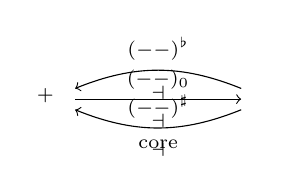
\begin{tikzpicture}[x=1.5em,y=1.1em]
  \node (L) at (0,0) {$\sSet^{+}$};
  \node (R) at (5.4,0) {$\sSet$};
  \draw[->] (4.7,0.35) to[bend right=22] node[pos=0.5,above]{$\scriptstyle(\text{--})^{\flat}$} node[pos=0.5,below=2pt]{$\scriptstyle\dashv$} (0.7,0.35);
  \draw[->] (0.7,0) -- node[pos=0.5,above]{$\scriptstyle(\text{--})_{0}$} node[pos=0.5,below=2pt]{$\scriptstyle\dashv$} (4.7,0);
  \draw[->] (4.7,-0.35) to[bend left=22] node[pos=0.5,above]{$\scriptstyle(\text{--})^{\sharp}$} node[pos=0.5,below=2pt]{$\scriptstyle\dashv$} (0.7,-0.35);
  \node at (2.7,-1.5) {$\scriptstyle\mathrm{core}$};
\end{tikzpicture}
\end{center}
\end{definition}

\trLeftAdjoint{} $(-)^{\flat}$ 给出\trSimplicialSet{}的\textbf{极小标记}（minimal
marking），其中只有退化\trSimplex{}被标记；\trRightAdjoint{} $(-)^{\sharp}$ 给出
\textbf{极大标记}（maximal marking），一切\trSimplex{}都被标记。这一函子还有一个
更进一层的\trRightAdjoint，它把一个\trMarkedSimplicialSet{}送到其\textbf{核}（core）：
即一个\trSimplicialSet{}，与原来具有相同的顶点，由那些诸面同样被标记的带标记\trSimplex{}所
组成。

在多种场合下，把 $\sSet$ 与刚刚引入的两支通往 $\sSet^{+}$ 的全忠实嵌入中的
某一者相认同是便利的。除非另有指明，默认约定是把\trSimplicialSet{}与其极小标记相
认同。特别地，在此约定下，我们可以自由地把标准\trSimplex{}及其子空间视为极小
标记的\trMarkedSimplicialSet{}。

为简便地引入其他\trMarkedSimplicialSet{}，下述术语是便利的：

\begin{definition}\label{def:regular-entire-inclusions}
\trMarkedSimplicialSet{}之间的一个包含 $U\hookrightarrow V$ 是：
\begin{itemize}
\item \textbf{正则的}（regular），记作 $U\hookrightarrow_{r}V$，若 $U$ 中的
  薄\trSimplex{}在 $V$ 中被创造；
\item \textbf{整的}（entire），记作 $U\hookrightarrow_{e}V$，若该映射在底%
  \trSimplicialSet{}上是\trIsomorphism（或更常见地，是恒同），此时 $U$ 与
  $V$ 之间的唯一差别在于 $V$ 带有更多的带标记\trSimplex{}。
\end{itemize}
\end{definition}

例如，对每个 $n\ge 1$，我们把\textbf{带标记\trSimplex}（marked simplex）
$\Delta[n]_{t}$ 定义为极小标记\trSimplex{} $\Delta[n]$ 的整扩张，后者还标记
最高维非退化\trSimplex{}。

\begin{notation}[带标记\trSimplex{}范畴]\label{not:marked-simplex-category}
设 $t\Delta\hookrightarrow\sSet^{+}$ 表示由极小标记\trSimplex{} $\Delta[n]$
（$n\ge 0$）连同带标记\trSimplex{} $\Delta[n]_{t}$（$n\ge 1$）所张成的全子范畴。
它可由第 1 章中的\cref{not:simplex-category} 的\trSimplex{}范畴 $\Delta$ 构建
如下：
\begin{itemize}
\item 添入对象 $[n]_{t}$，对 $n\ge 1$；
\item 添入映射 $\phi\colon[n]\to[n]_{t}$，对 $n\ge 1$；以及
  $\xi^{i}\colon[n+1]_{t}\to[n]$，对 $n\ge 0$ 与 $0\le i\le n$；并且
\item 强加关系 $\xi^{i}\phi=\sigma^{i}$ 与%
  $\sigma^{i}\xi^{j+1}=\sigma^{j}\xi^{i}$，对 $i\le j$。\footnote{Viktoriya Ozornova 与 Martina
  Rovelli 向我们指出：最后这一族关系在原始文献 \cite{bib122} 中被遗漏了，
  但本应包含在内。一个修正后的定义见 \cite[1.1]{bib89}。}
\end{itemize}
\end{notation}

对一个\trMarkedSimplicialSet{} $X$，映射 $\Delta[n]\to X$ 与 $\Delta[n]_{t}\to X$ 分别
参数化 $X$ 中的 $n$-\trSimplex{}与 $X$ 中的带标记 $n$-\trSimplex{}。这定义了一个\trCanonical{}%
嵌入 $\sSet^{+}\hookrightarrow\mathcal{S}et^{t\Delta^{\mathrm{op}}}$，容易
看出它是\trFullyFaithful。此外：

\begin{proposition}\label{prop:reflective-embedding}
存在一个反射嵌入（reflective embedding）
\begin{center}
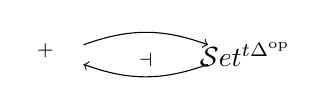
\begin{tikzpicture}[x=1.5em,y=1.1em]
  \node (L) at (0,0) {$\sSet^{+}$};
  \node (R) at (4.8,0) {$\mathcal{S}et^{t\Delta^{\mathrm{op}}}$};
  \draw[->] (0.9,0.32) to[bend left=20] (3.9,0.32);
  \draw[->] (3.9,-0.32) to[bend left=20] node[pos=0.5,above]{$\scriptstyle\dashv$} (0.9,-0.32);
\end{tikzpicture}
\end{center}
其
\begin{enumerate}[label=(\roman*)]
\item 本质像由那些预层（presheaf）$F$ 组成：其分量映射
  $-\circ\phi\colon F_{[n]_{t}}\to F_{[n]}$ 都是\trMonomorphism；并且
\item 左伴随构造为：把集合 $F_{[n]_{t}}$ 替换为映射
  $-\circ\phi\colon F_{[n]_{t}}\to F_{[n]}$ 的像。
\end{enumerate}
\end{proposition}

\emph{从而，$\sSet^{+}$ 是一个局部有限可表现（locally finitely
presentable）的范畴，特别地是完备且余完备的：其诸\trLimit{}作为预层逐点
构造，而其诸\trColimit{}则通过把反射作用施加于预层的逐点余极限而构造。}

{\tolerance=3000\emergencystretch=3em%
用更初等的话来说：\trMarkedSimplicialSet{}的诸\trLimit{}与诸\trColimit{}由底%
\trSimplicialSet{}函子 $(-)_{0}\colon\sSet^{+}\to\sSet$ 所创造。\trLimit{}%
中的一个\trSimplex{}被标记，当且仅当它的\emph{每一个}分量——通过沿\trLimit{}
\trCone{}的诸腿作复合而定义——都是带标记\trSimplex{}。\trColimit{}中的一个\trSimplex{}%
被标记，若它沿余极限锥的任一条腿的\emph{任一}\trLifting{}是带标记\trSimplex{}。(ii) 中
的反射是一种「命题截断」（propositional truncation）：它记住哪些\trSimplex{}应当
被标记，而忘掉指示其缘由的数据。\par}

\begin{proof}
$t\Delta$ 中诸算子在一个预层 $F\in\mathcal{S}et^{t\Delta^{\mathrm{op}}}$ 上的
右作用，赋予 $F$ 的诸元素之集一个\trMarkedSimplicialSet{}的结构，唯一的例外是一个条件：
即带标记 $n$-\trSimplex{}构成 $n$-\trSimplex{}的一个子集。这解释了出现于 (i) 中的条件
与出现于 (ii) 中的构造。由此可知：\trMarkedSimplicialSet{}乃是一个有限极限草图
（finite limit sketch）之诸模型的\trCategory，从而构成一个局部有限可表现的%
\trCategory。完备且余完备的\trCategory{}的任何反射全子范畴，都按陈述中所
构造的方式继承极限（例如见 \cite[4.5.15]{bib104}）。
\end{proof}

附录 C 中的\cref{lem:mono-epi-reedy-sset}可以推广到\trMarkedSimplicialSet{}的情形，
如下：

\begin{lemma}\label{lem:mono-marked-cellularly-generated}
$\sSet^{+}$ 中的诸\trMonomorphism{}由
\[
\{\partial\Delta[n]\hookrightarrow_{r}\Delta[n]\}_{n\ge 0}
\;\cup\;
\{\Delta[n]\hookrightarrow_{e}\Delta[n]_{t}\}_{n\ge 1}
\]
\trCell{}式生成。
\end{lemma}

\begin{proof}
见\cref{ex:prove-lem-mono-generated}。
\end{proof}

一个\trMarkedSimplicialSet{}是一个带有足够结构的\trSimplicialSet{}，使我们得以谈论所有维数上\trSimplex{}%
的复合。一个复状单纯集是一个\trMarkedSimplicialSet{}，其中复合存在，而且复合的诸薄见证
者相复合而定义薄\trSimplex{}——这一结合性条件最终蕴含：薄\trSimplex{}是某种意义下的%
\trEquivalence，其确切含义在\cref{lem:marked-edges-equivalences}与%
\cref{dig:saturation-higher-simplices}中给出。下述这一
形式的复状单纯集定义（旧称\emph{弱}复状单纯集）归于 \trVerity{} \cite{bib129}，它
修改了早先归于 Street \cite{bib120} 的一个等价表述。\trVerity{}的修改聚焦
于一类特别的\emph{$k$-容许 $n$-\trSimplex{}}：它们是把自己的第 $k$ 面展现为
第 $(k+1)$ 面与第 $(k-1)$ 面之复合的薄 $n$-\trSimplex{}——在 $0<k<n$ 的情形。

而当 $k=0$ 或 $k=n$ 时，一个 $k$-容许 $n$-\trSimplex{}分别见证最初一对面之间或
最后一对面之间的\trEquivalence。

\begin{definition}[$k$-容许 $n$-\trSimplex{}]\label{def:k-admissible-simplex}
对 $n\ge 1$ 与 $0\le k\le n$，\textbf{$k$-容许 $n$-\trSimplex{}} $\Delta^{k}[n]$
是标准 $n$-\trSimplex{}的整超集，其中某些附加的面被标记为薄：$\Delta^{k}[n]$ 中
的一个非退化 $m$-\trSimplex{}是薄的，当且仅当它包含 $\{k-1,k,k+1\}\cap[n]$ 中的
全部顶点。薄面特别包括：
\begin{itemize}
\item 最高维的 $n$-\trSimplex{}；
\item 除第 $(k-1)$ 个、第 $k$ 个与第 $(k+1)$ 个面之外的一切余维一面；
\item 当 $0<k<n$ 时由 $\{k-1,k,k+1\}$ 张成的 2-\trSimplex{}，\yizhu{原书于此印作
  「when $0\le k\le n$」，然 $k=0$ 或 $k=n$ 时并无由 $\{k-1,k,k+1\}$ 张成的
  2-\trSimplex{}（该集含越界顶点），按文义疑为 $0<k<n$ 之误，此处径改。——译者注}或当 $k=0$ 或 $k=n$ 时由 $\{k-1,k,k+1\}\cap[n]$ 张成的边。
\end{itemize}
\end{definition}

在画\trMarkedSimplicialSet{}的图时，我们用符号「$\simeq$」装饰带标记\trSimplex{}，用
「$\sim$」装饰带标记的边。我们的图还采用一个约定，规定栖居于一个无标记
$n$-\trSimplex{}中的胞腔的方向。遵循 Street 在其「定向\trSimplex{}之代数」\cite{bib120}
中引入的组合学，我们把一个 $n$-\trSimplex{}视为一个 $n$-胞腔，从其诸奇数号面的
粘贴复合指向其诸偶数号面的粘贴复合。注意这与既已通用的约定相容，即把\trSimplicialSet{}%
中的一个 1-\trSimplex{}描绘成一支从其第 1 面（第 0 个顶点）指向其第 0 面（第 1 个
顶点）的箭头。

\begin{example}[低维容许\trSimplex{}]\label{exa:admissible-low-dimensions}
\begin{enumerate}[label=(\roman*)]
\item 对 $n=1$，两个容许\trSimplex{} $\Delta^{0}[1]$ 与 $\Delta^{1}[1]$ 都等于薄
  1-\trSimplex{} $\Delta[1]_{t}=\Delta[1]^{\sharp}$。一个映射
  $\Delta[1]^{\sharp}\to A$ 被诠释为在其像中定义两个顶点之间的一个%
  \trEquivalence。
\item 对 $n=2$，容许\trSimplex{} $\Delta^{1}[2]$ 等于薄 2-\trSimplex{} $\Delta[2]_{t}$。
  一个映射 $\Delta^{1}[2]\to A$ 被诠释为指明：$\{02\}$-边的像是 $\{01\}$-边
  与 $\{12\}$-边之像的一个复合。相比之下，$\Delta^{0}[2]$ 与 $\Delta^{2}[2]$
  各有一条带标记的边，也有一个带标记的 2-\trSimplex{}，如下图所示：
\begin{center}
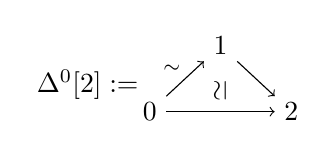
\begin{tikzpicture}[x=1.6em,y=1.4em]
  \node at (-1.4,0.7) {$\Delta^{0}[2]:=$};
  \node (v0) at (0,0) {$0$};
  \node (v1) at (1.6,1.7) {$1$};
  \node (v2) at (3.2,0) {$2$};
  \draw[->] (v0) -- (v1);
  \node at (0.5,1.1) {$\scriptstyle\sim$};
  \draw[->] (v1) -- (v2);
  \draw[->] (v0) -- (v2);
  \node[rotate=90] at (1.6,0.55) {$\simeq$};
\end{tikzpicture}
\qquad
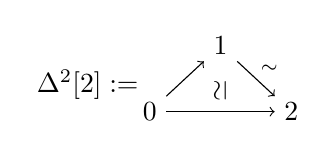
\begin{tikzpicture}[x=1.6em,y=1.4em]
  \node at (-1.4,0.7) {$\Delta^{2}[2]:=$};
  \node (v0) at (0,0) {$0$};
  \node (v1) at (1.6,1.7) {$1$};
  \node (v2) at (3.2,0) {$2$};
  \draw[->] (v0) -- (v1);
  \draw[->] (v1) -- (v2);
  \node at (2.7,1.1) {$\scriptstyle\sim$};
  \draw[->] (v0) -- (v2);
  \node[rotate=90] at (1.6,0.55) {$\simeq$};
\end{tikzpicture}
\end{center}
  一个映射 $\Delta^{0}[2]\to A$ 见证 $\{12\}$-边之像与 $\{02\}$-边之像之间
  的一个\trEquivalence。
\item 对 $n=3$，容许\trSimplex{} $\Delta^{1}[3]$ 与 $\Delta^{2}[3]$ 分别有它们的
  第 3 面与第 0 面被标记，连同最高维的 3-\trSimplex{}，而无任何其他非退化面被
  标记。我们选择以一种能让我们看见全部余维一面的方式来画容许 3-\trSimplex{}：
\begin{center}
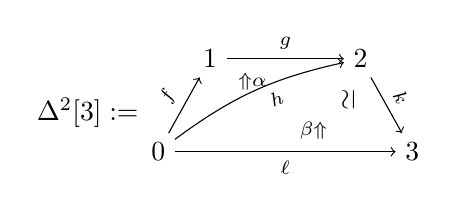
\begin{tikzpicture}[x=1.7em,y=1.4em]
  \node at (-1.5,1.0) {$\Delta^{2}[3]:=$};
  \node (v0) at (0,0) {$0$};
  \node (v3) at (5.4,0) {$3$};
  \node (v1) at (1.1,2.4) {$1$};
  \node (v2) at (4.3,2.4) {$2$};
  \draw[->] (v0) -- node[above,sloped]{$\scriptstyle f$} (v1);
  \draw[->] (v1) -- node[above]{$\scriptstyle g$} (v2);
  \draw[->] (v2) -- node[above,sloped]{$\scriptstyle k$} (v3);
  \draw[->] (v0) to[bend left=12] node[below,sloped,pos=0.6]{$\scriptstyle h$} (v2);
  \draw[->] (v0) -- node[below]{$\scriptstyle\ell$} (v3);
  \node[rotate=90] at (4.05,1.35) {$\simeq$};
  \node at (2.0,1.8) {$\scriptstyle\Uparrow\alpha$};
  \node at (3.3,0.55) {$\scriptstyle\beta\Uparrow$};
\end{tikzpicture}
\quad$\simeq$\quad
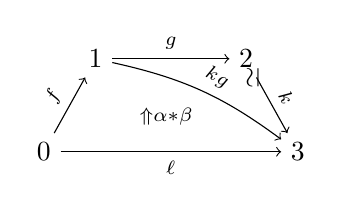
\begin{tikzpicture}[x=1.7em,y=1.4em]
  \node (v0) at (0,0) {$0$};
  \node (v3) at (5.4,0) {$3$};
  \node (v1) at (1.1,2.4) {$1$};
  \node (v2) at (4.3,2.4) {$2$};
  \draw[->] (v0) -- node[above,sloped]{$\scriptstyle f$} (v1);
  \draw[->] (v1) -- node[above]{$\scriptstyle g$} (v2);
  \draw[->] (v2) -- node[above,sloped]{$\scriptstyle k$} (v3);
  \draw[->] (v1) to[bend left=12] node[above,sloped,pos=0.55]{$\scriptstyle kg$} (v3);
  \draw[->] (v0) -- node[below]{$\scriptstyle\ell$} (v3);
  \node[rotate=90] at (4.45,1.9) {$\simeq$};
  \node at (2.6,0.9) {$\scriptstyle\Uparrow\alpha\ast\beta$};
\end{tikzpicture}
\end{center}
  这里我们对诸面加以标号，以便更好地描述一个映射 $\Delta^{2}[3]\to A$ 的
  诠释。它的第 0 面——其自身是一个容许\trSimplex{} $\Delta^{1}[2]$——见证边
  $\{13\}$ 是边 $\{12\}$ 与 $\{23\}$ 的一个复合。注意由于第 0 面是薄的，
  其第 1 边被诠释为 $g$ 与 $k$ 的复合 $kg$；出现于第 2 面中的 2-胞腔之
  边缘要与 $\beta$ 和 $\alpha$ 的粘贴复合之边缘相一致，正需要这一点。鉴于
  这一边缘条件以及薄的 3-\trSimplex{}，我们把第 2 面诠释为右图所描绘的第 1 面与
  第 3 面的粘贴复合。

  容许\trSimplex{} $\Delta^{0}[3]$ 有它的第 2 面与第 3 面被标记，连同最高维的
  3-\trSimplex{}，以及边 $\{01\}$。对偶地，$\Delta^{3}[3]$ 有它的第 0 面与第 1 面
  被标记，连同最高维的 3-\trSimplex{}，以及边 $\{23\}$。
\begin{center}
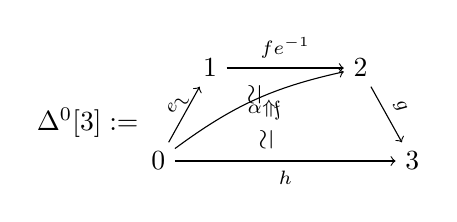
\begin{tikzpicture}[x=1.7em,y=1.4em]
  \node at (-1.5,1.0) {$\Delta^{0}[3]:=$};
  \node (v0) at (0,0) {$0$};
  \node (v3) at (5.4,0) {$3$};
  \node (v1) at (1.1,2.4) {$1$};
  \node (v2) at (4.3,2.4) {$2$};
  \draw[->] (v0) -- node[above,sloped]{$\scriptstyle e$} (v1);
  \node at (0.5,1.5) {$\scriptstyle\sim$};
  \draw[->] (v1) -- node[above]{$\scriptstyle fe^{-1}$} (v2);
  \draw[->] (v2) -- node[above,sloped]{$\scriptstyle g$} (v3);
  \draw[->] (v0) to[bend left=12] node[below,sloped,pos=0.6]{$\scriptstyle f$} (v2);
  \draw[->] (v0) -- node[below]{$\scriptstyle h$} (v3);
  \node[rotate=90] at (2.05,1.7) {$\simeq$};
  \node[rotate=90] at (2.3,0.55) {$\simeq$};
  \node at (2.2,1.35) {$\scriptstyle\alpha\Uparrow$};
\end{tikzpicture}
\quad$\simeq$\quad
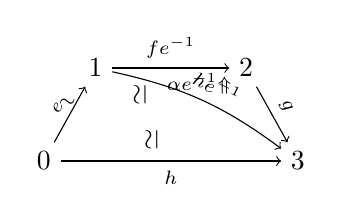
\begin{tikzpicture}[x=1.7em,y=1.4em]
  \node (v0) at (0,0) {$0$};
  \node (v3) at (5.4,0) {$3$};
  \node (v1) at (1.1,2.4) {$1$};
  \node (v2) at (4.3,2.4) {$2$};
  \draw[->] (v0) -- node[above,sloped]{$\scriptstyle e$} (v1);
  \node at (0.5,1.5) {$\scriptstyle\sim$};
  \draw[->] (v1) -- node[above]{$\scriptstyle fe^{-1}$} (v2);
  \draw[->] (v2) -- node[above,sloped]{$\scriptstyle g$} (v3);
  \draw[->] (v1) to[bend left=12] node[above,sloped,pos=0.55]{$\scriptstyle he^{-1}$} (v3);
  \node at (3.3,2.0) {$\scriptstyle\alpha e^{-1}\Uparrow$};
  \draw[->] (v0) -- node[below]{$\scriptstyle h$} (v3);
  \node[rotate=90] at (2.05,1.7) {$\simeq$};
  \node[rotate=90] at (2.3,0.55) {$\simeq$};
\end{tikzpicture}
\end{center}
  一个映射 $\Delta^{0}[3]\to A$ 被诠释为见证分别占据第 0 面与第 1 面的那对
  非薄 2-\trSimplex{}之间的一个\trEquivalence。
\end{enumerate}
\end{example}

\begin{definition}\label{def:complicial-set}
一个\textbf{复状单纯集}是一个\trMarkedSimplicialSet{} $A$：对由以下两族映射给出的%
\textbf{初等带标记\trAnodyneExtension}（elementary marked anodyne extensions），它都
容有\trExtension。
\begin{enumerate}[label=(\roman*)]
\item \textbf{复状号角扩张}（complicial horn extensions）
\begin{rveq}\label{eq:complicial-horn-extension}
\begin{tikzpicture}[x=1.6em,y=1.4em]
  \node (lt) at (0,1.2) {$\Lambda^{k}[n]$};
  \node (rt) at (2.8,1.2) {$A$};
  \node (lb) at (0,-1.2) {$\Delta^{k}[n]$};
  \draw[->] (lt) -- (rt);
  \draw[right hook->] (lb) -- (lt);
  \node at (-0.45,0) {$\scriptstyle r$};
  \draw[->,dashed] (0.45,-1.0) -- (2.35,1.0);
\end{tikzpicture}
\qquad \text{对\quad $n\ge 1$，\ $0\le k\le n$}%
\end{rveq}
是诸\textbf{$k$-容许 $n$-号角}的正则包含。一个内容许 $n$-号角参数化一对
$(n-1)$-\trSimplex{}的「容许复合」。该\trExtension{}定义了一个复合的 $(n-1)$-\trSimplex{}，连同一个薄的 $n$-\trSimplex{}见证者。
\item \textbf{复状薄性扩张}（complicial thinness extensions）
\begin{rveq}\label{eq:complicial-thinness-extension}
\begin{tikzpicture}[x=1.6em,y=1.4em]
  \node (lt) at (0,1.2) {$\Delta^{k}[n]'$};
  \node (rt) at (2.8,1.2) {$A$};
  \node (lb) at (0,-1.2) {$\Delta^{k}[n]''$};
  \draw[->] (lt) -- (rt);
  \draw[right hook->] (lb) -- (lt);
  \draw[->,dashed] (0.45,-1.0) -- (2.35,1.0);
\end{tikzpicture}
\qquad \text{对\quad $n\ge 2$，\ $0\le k\le n$}%
\end{rveq}
是 $\Delta^{k}[n]$ 的两个整超集之间的\trEntireInclusion。\trMarkedSimplicialSet{} $\Delta^{k}[n]'$
由 $\Delta^{k}[n]$ 再标记第 $(k-1)$ 面与第 $(k+1)$ 面而得，而
$\Delta^{k}[n]''$ 则标记了全部余维一面。这一\trExtension{}问题要求：但凡
容许号角中的可复合\trSimplex{}对是薄的，任何复合便也是薄的。
\end{enumerate}
\end{definition}

\begin{example}[复状号角扩张]\label{exa:complicial-horn-extensions}
对 $\Lambda^{2}[4]\hookrightarrow_{r}\Delta^{2}[4]$ 而言，号角中的诸非薄
余维一面给出左图所示的两个具有公共面的 3-\trSimplex{}，而它们的复合则是右图所示的
一个 3-\trSimplex{}。
\begin{center}
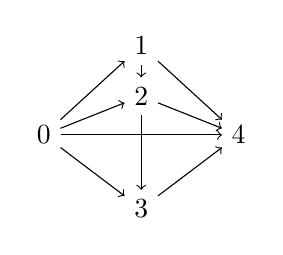
\begin{tikzpicture}[x=1.6em,y=1.4em]
  \node (v1) at (2.2,3.2) {$1$};
  \node (v2) at (2.2,1.9) {$2$};
  \node (v0) at (0,0.9) {$0$};
  \node (v4) at (4.4,0.9) {$4$};
  \node (v3) at (2.2,-1.0) {$3$};
  \draw[->] (v0) -- (v1);
  \draw[->] (v1) -- (v2);
  \draw[->] (v0) -- (v2);
  \draw[->] (v1) -- (v4);
  \draw[->] (v2) -- (v4);
  \draw[->] (v0) -- (v4);
  \draw[->] (v0) -- (v3);
  \draw[->] (v2) -- (v3);
  \draw[->] (v3) -- (v4);
\end{tikzpicture}
\qquad
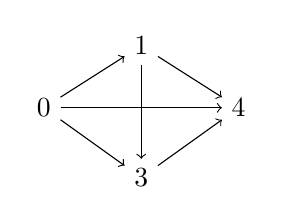
\begin{tikzpicture}[x=1.6em,y=1.4em]
  \node (v1) at (2.2,2.8) {$1$};
  \node (v0) at (0,1.2) {$0$};
  \node (v4) at (4.4,1.2) {$4$};
  \node (v3) at (2.2,-0.6) {$3$};
  \draw[->] (v0) -- (v1);
  \draw[->] (v0) -- (v4);
  \draw[->] (v0) -- (v3);
  \draw[->] (v1) -- (v4);
  \draw[->] (v1) -- (v3);
  \draw[->] (v3) -- (v4);
\end{tikzpicture}
\end{center}
把右手边的\trSimplex{}——即 2-容许 4-\trSimplex{}的第 2 面——诠释为第 3 面与第 1 面的
一个复合是有意义的，因为下列诸\trSimplex{}是薄的：
\begin{center}
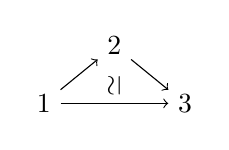
\begin{tikzpicture}[x=1.5em,y=1.3em]
  \node (a) at (0,0) {$1$};
  \node (c) at (3.4,0) {$3$};
  \node (b) at (1.7,1.6) {$2$};
  \draw[->] (a) -- (b);
  \draw[->] (b) -- (c);
  \draw[->] (a) -- (c);
  \node[rotate=90] at (1.7,0.5) {$\simeq$};
\end{tikzpicture}
\qquad
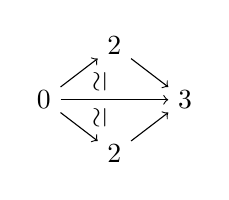
\begin{tikzpicture}[x=1.5em,y=1.3em]
  \node (l) at (0,0) {$0$};
  \node (r) at (3.4,0) {$3$};
  \node (t) at (1.7,1.5) {$2$};
  \node (b) at (1.7,-1.5) {$2$};
  \draw[->] (l) -- (t);
  \draw[->] (t) -- (r);
  \draw[->] (l) -- (r);
  \draw[->] (l) -- (b);
  \draw[->] (b) -- (r);
  \node[rotate=90] at (1.35,0.5) {$\simeq$};
  \node[rotate=90] at (1.35,-0.5) {$\simeq$};
\end{tikzpicture}
\qquad
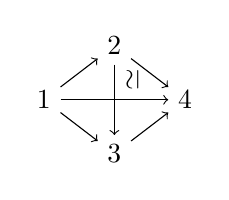
\begin{tikzpicture}[x=1.5em,y=1.3em]
  \node (l) at (0,0) {$1$};
  \node (r) at (3.4,0) {$4$};
  \node (t) at (1.7,1.5) {$2$};
  \node (b) at (1.7,-1.5) {$3$};
  \draw[->] (l) -- (t);
  \draw[->] (t) -- (r);
  \draw[->] (l) -- (b);
  \draw[->] (b) -- (r);
  \draw[->] (l) -- (r);
  \draw[->] (t) -- (b);
  \node[rotate=90] at (2.15,0.55) {$\simeq$};
\end{tikzpicture}
\end{center}
\end{example}

我们把由诸初等带标记\trAnodyneExtension\trCell{}式生成的那些映射称作\textbf{带标记%
\trAnodyneExtension}（marked anodyne extensions）。例如，把求解第 1 章中的%
\cref{ex:free-living-isomorphism} 的论证稍加推广：

\begin{lemma}\label{lem:marked-anodyne-free-isomorphism}
把带标记 1-\trSimplex{}映入极大标记同构的包含
$\qcTwo^{\sharp}\hookrightarrow\qcInt^{\sharp}$ 是一支带标记\trAnodyneExtension，单射
$\qcOne\hookrightarrow\qcInt^{\sharp}$ 亦然。
\end{lemma}

\begin{proof}
见\cref{ex:prove-lem-anodyne}。
\end{proof}

\begin{definition}\label{def:complicial-isofibration}
\trMarkedSimplicialSet{}之间的一个映射是一个\textbf{复状等价纤维化}（complicial
isofibration），若它对诸初等带标记\trAnodyneExtension{}具有右\trLifting{}性质，且其
定义域与余定义域都是复状单纯集。
\end{definition}

由\cref{ex:thinness-for-free}，复状单纯集之间的一个带标记映射是一个复状
等价纤维化，当且仅当它对诸复状号角扩张有\trLifting——诸复状薄性扩张则
自动白得。由附录 C 中的\cref{lem:right-lifting-closure}，复状等价纤维化
随之对一切带标记\trAnodyneExtension{}都具有右\trLifting{}性质。诸\textbf{%
\trTrivialFibration}——被定义为对诸\trMonomorphism{}有\trLifting{}的那些%
\trMarkedSimplicialSet{}之间的映射——也在复状等价纤维化之列，一如%
\cref{lem:mono-marked-cellularly-generated} 所刻画的那样。

「复状单纯集」一词的原初含义指的只是我们如今称作\emph{严格}的那一特定
品种。

\begin{definition}\label{def:strict-complicial-set}
一个\textbf{严格复状单纯集}（strict complicial set）是一个沿诸初等带标记%
\trAnodyneExtension \eqref{eq:complicial-horn-extension} 与
\eqref{eq:complicial-thinness-extension} 容有唯一\trExtension{}的带标记%
\trSimplicialSet{}。
\end{definition}

在手稿 \cite{bib128} 中，\trVerity{}证明了：严格复状单纯集恰是那些作为
严格 $\omega$-范畴的 Street 神经的\trMarkedSimplicialSet{}，从而解决了 Roberts 与
Street 的一个猜想。在本手稿中，我们主要利用\trMarkedSimplicialSet{}来简化关于
拟范畴中\trIsomorphism{}与拟范畴之间的\trEquivalence{}的诸结果的证明。在发展出期间所需的若干组合构造之后，
我们将在 D.4 节与 D.5 节中更明确地讨论这一话题。

\begin{definition}\label{def:n-trivial}
一个\trMarkedSimplicialSet{} $X$ 是 \textbf{$n$-平凡}（$n$-trivial）的，若所有 $r>n$
的 $r$-\trSimplex{}都被标记。
\end{definition}

$n$-平凡\trMarkedSimplicialSet{}的全子范畴在\trMarkedSimplicialSet{}的\trCategory{}中既是反射的
（reflective）又是余反射的（coreflective）：
\begin{center}
\begin{tikzpicture}[x=1.5em,y=1.1em]
  \node (L) at (0,0) {$n\text{-}\sSet^{+}$};
  \node (R) at (4.8,0) {$\sSet^{+}$};
  \draw[->] (3.9,0.32) to[bend right=20] node[pos=0.5,above=10pt]{$\scriptstyle\mathrm{trv}_{n}$} node[pos=0.5,above=1pt]{$\scriptstyle\dashv$} (0.9,0.32);
  \draw[right hook->] (0.7,0) -- (4.1,0);
  \draw[->] (3.9,-0.32) to[bend left=20] node[pos=0.5,below=1pt]{$\scriptstyle\dashv$} node[pos=0.5,below=10pt]{$\scriptstyle\mathrm{core}_{n}$} (0.9,-0.32);
\end{tikzpicture}
\end{center}
也就是说，\textbf{$n$-平凡化}（$n$-trivialization）在 $\sSet^{+}$ 上定义
了一个\trIdempotent{}\trMonad，其单位是\trMarkedSimplicialSet{} $X$ 进入\trMarkedSimplicialSet{}
$\mathrm{trv}_{n}X$ 的\trEntireInclusion{} $X\hookrightarrow_{e}\mathrm{trv}_{n}X$——
后者在维数 $1,\dots,n$ 中与 $X$ 带有相同的带标记\trSimplex{}，而所有更高维的%
\trSimplex{}都「被弄薄」。一个复状单纯集是 $n$-平凡的，若此映射是一个%
\trIsomorphism。

$n$-\textbf{核}（$n$-core）$\mathrm{core}_{n}X$——由限制在那些于 $X$ 中
维数高于 $n$ 的诸面皆为薄的\trSimplex{}上而定义——定义了一个\trIdempotent{}余
单子（comonad），其余单位是正则包含 $\mathrm{core}_{n}X\hookrightarrow_{r}X$。
同样地，一个复状单纯集是 $n$-平凡的，恰好当此映射是一个\trEquivalence。对如
此产生的单子–余单子对而言，这些函子是一对\trAdjunction：
$\mathrm{trv}_{n}\dashv\mathrm{core}_{n}$。

诸 $n$-平凡\trMarkedSimplicialSet{}之子范畴的包含拥有\trAdjunction
\begin{center}
\begin{tikzpicture}[x=1.5em,y=1.1em]
  \node (S) at (0,0) {$\sSet$};
  \node (A) at (2.8,0) {$0\text{-}\sSet^{+}$};
  \node (D1) at (5.2,0) {$\subset\cdots\subset$};
  \node (B) at (7.8,0) {$(n{-}1)\text{-}\sSet^{+}$};
  \node (C) at (11.0,0) {$n\text{-}\sSet^{+}$};
  \node (D2) at (13.4,0) {$\subset\cdots\subset$};
  \node (T) at (15.8,0) {$\sSet^{+}$};
  \draw[->] (S) -- node[pos=0.5,above]{$\scriptstyle(\text{--})^{\sharp}$} node[pos=0.5,below]{$\scriptstyle\simeq$} (A);
  \draw[->] (C) to[bend right=22] node[pos=0.5,above=10pt]{$\scriptstyle\mathrm{trv}_{n-1}$} node[pos=0.5,above=1pt]{$\scriptstyle\dashv$} (B);
  \draw[right hook->] (8.5,0) -- (10.3,0);
  \draw[->] (C) to[bend left=22] node[pos=0.5,below=1pt]{$\scriptstyle\dashv$} node[pos=0.5,below=10pt]{$\scriptstyle\mathrm{core}_{n-1}$} (B);
\end{tikzpicture}
\end{center}
复状单纯集的 $n$-核仍是一个复状单纯集，但 $n$-平凡化函子——它只是在相应的
维数标记\trSimplex{}而不改动底\trSimplicialSet——却不必然保持复状单纯集（见
\cref{ex:n-core-complicial}）。

\begin{remark}[奇对偶]\label{rem:odd-dual}
回顾：一个\trSimplicialSet{} $X$ 的\textbf{\trOppositeSimplicialSet}，是把
$X$ 沿对合 $(-)^{\mathrm{op}}\colon\Delta\to\Delta$——它反转每个序数中的
排序——重新标号而得的\trSimplicialSet{}。这一运算可以自然的方式扩张到\trMarkedSimplicialSet{}上：
在 $X^{\mathrm{op}}$ 中标记一个 $n$-\trSimplex{}，恰好当 $X$ 中相应的 $n$-\trSimplex{}被
标记。然而请注意，按 Street 对 $n$-\trSimplex{}的诠释——它编码一个 $n$ 维态射，
从其诸奇数 $(n-1)$ 维面的复合指向其诸偶数 $(n-1)$ 维面的复合——这一运算
并非简单地反转\trMarkedSimplicialSet{}中「所有胞腔的方向」。毋宁说，它只反转\emph{奇数}
维胞腔中所有\trSimplex{}的方向，而在所有偶数维胞腔中保持方向不变。因此，我们把
这一顶点重排构造称作\trMarkedSimplicialSet{}的\textbf{奇对偶}（odd dual）。
\end{remark}

我们以一段关于复状单纯集之间\trEquivalence{}的讨论作结。

\begin{definition}[复状单纯集的等价]\label{def:complicial-equivalences}
复状单纯集之间的一个映射 $f\colon A\to B$ 是一个\textbf{\trEquivalence}，
若它扩张成一份以带标记 1-\trSimplex{} $\Delta[1]^{\sharp}$ 为\trInterval{}的%
\trHomotopyEquivalence{}数据：\footnote{大体上由
\cref{lem:marked-anodyne-free-isomorphism}，复状单纯集间的\trEquivalence{}%
本可改用带标记\trHomotopyCoherentIsomorphism{} $\qcInt^{\sharp}$ 来定义
（见\cref{cor:complicial-equivalences-hoc}）。但复状单纯集这一高阶范畴模型的优势之一在于：正确的%
\trEquivalence{}概念可以用带标记 1-\trSimplex{}这份更简单的数据来定义。}也就是说，
若存在映射
$g\colon B\to A$，连同
\begin{center}
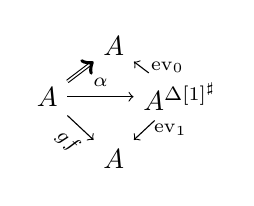
\begin{tikzpicture}[x=1.6em,y=1.4em]
  \node (At) at (1.5,2.4) {$A$};
  \node (Al) at (0,1.1) {$A$};
  \node (M) at (3.0,1.1) {$A^{\Delta[1]^{\sharp}}$};
  \node (Ab) at (1.5,-0.5) {$A$};
  \draw[double,->] (Al) -- (At);
  \draw[->] (Al) -- node[above]{$\scriptstyle\alpha$} (M);
  \draw[->] (M) -- node[right]{$\scriptstyle\mathrm{ev}_{0}$} (At);
  \draw[->] (M) -- node[right]{$\scriptstyle\mathrm{ev}_{1}$} (Ab);
  \draw[->] (Al) -- node[below,sloped]{$\scriptstyle gf$} (Ab);
\end{tikzpicture}
\qquad 与 \qquad
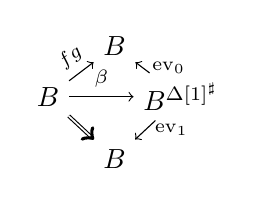
\begin{tikzpicture}[x=1.6em,y=1.4em]
  \node (Bt) at (1.5,2.4) {$B$};
  \node (Bl) at (0,1.1) {$B$};
  \node (M) at (3.0,1.1) {$B^{\Delta[1]^{\sharp}}$};
  \node (Bb) at (1.5,-0.5) {$B$};
  \draw[->] (Bl) -- node[above,sloped]{$\scriptstyle fg$} (Bt);
  \draw[->] (Bl) -- node[above]{$\scriptstyle\beta$} (M);
  \draw[->] (M) -- node[right]{$\scriptstyle\mathrm{ev}_{0}$} (Bt);
  \draw[->] (M) -- node[right]{$\scriptstyle\mathrm{ev}_{1}$} (Bb);
  \draw[double,->] (Bl) -- (Bb);
\end{tikzpicture}
\end{center}
\end{definition}

复状单纯集间等价的数据经转置便给出「带标记\trHomotopyEquivalence」这一更
一般概念的一个实例——对于后者，我们去掉\trMarkedSimplicialSet{}须为复状单纯集的要求。

\begin{definition}\label{def:marked-homotopy}
映射对 $f,g\colon X\to Y$ 之间的一个\textbf{带标记\trHomotopy}（marked
homotopy），由一个映射 $\alpha\colon X\times\Delta[1]^{\sharp}\to Y$ 给出，
它沿端点包含 $X+X\hookrightarrow_{r}X\times\Delta[1]^{\sharp}$ 的限制分别
为映射 $f$ 与 $g$。当 $X$ 与 $Y$ 是极小标记\trSimplicialSet{}时，一个映射
$X\times\Delta[1]\to Y$ 可\trExtension{}为映射
$X\times\Delta[1]^{\sharp}\to Y$，恰好当对每个 0-\trSimplex{} $x\in X$，1-\trSimplex{}
$(x\sigma^{0},\mathrm{id}_{[1]})\in X\times\Delta[1]^{\sharp}$ 被送到 $Y$
的一个退化、从而被标记的 1-\trSimplex{}。\footnote{\trMarkedSimplicialSet{}的\trCartesianProduct{}将在%
\cref{prop:marked-cartesian-closed}中更详细地描述。}
\end{definition}

\textbf{带标记\trHomotopyEquivalence}（marked homotopy equivalence）由
如下数据构成：
\begin{itemize}
\item 一对带标记映射 $f\colon X\to Y$ 与 $g\colon Y\to X$；以及
\item 一对带标记\trHomotopy{} $\alpha\colon X\times\Delta[1]^{\sharp}\to X$
  与 $\beta\colon Y\times\Delta[1]^{\sharp}\to Y$，分别是 $\mathrm{id}_{X}$
  与 $gf$ 之间、以及 $fg$ 与 $\mathrm{id}_{Y}$ 之间的\trHomotopy。
\end{itemize}

当 $X$ 与 $Y$ 是复状单纯集时，带标记\trHomotopy{}可以反转与复合。即便情形
并非如此，我们也容许自己不经说明地反转构成一个带标记\trHomotopyEquivalence{}%
的那些带标记\trHomotopy{}的方向。

\begin{digression}[复状单纯集的 \trVerity{}模型结构]\label{dig:verity-model-structure}
\trMarkedSimplicialSet{}的\trCategory{}带有一个\trCartesianClosed、余纤维性生成的%
\trModelStructure，其\trFibrant{}对象恰是诸复状单纯集，而其诸余纤维化恰为诸%
\trMonomorphism{} \cite[\S6.2-4]{bib129}。在纤维性对象之间，诸\trFibration{}%
与诸\trWeakEquivalence{}恰是上文定义的复状等价纤维化类与\trEquivalence{}类。
在以下各节中，我们直接对纤维性对象范畴验证其中的许多性质，只把%
\trModelStructure{}本身的验证留给文献——它由 Jeff Smith 定理得出。
\end{digression}

\subsection*{练习}

\begin{exercise}\label{ex:prove-lem-mono-generated}
证明\cref{lem:mono-marked-cellularly-generated}。
\end{exercise}

\begin{exercise}\label{ex:maximally-marked-kan}
证明：一个极大标记\trSimplicialSet{}定义一个复状单纯集，当且仅当其底\trSimplicialSet{}%
是一个\trKanComplex。
\end{exercise}

\begin{exercise}\label{ex:prove-lem-anodyne}
证明\cref{lem:marked-anodyne-free-isomorphism}。
\end{exercise}

\begin{exercise}\label{ex:thinness-for-free}
设 $f\colon A\to B$ 是\trMarkedSimplicialSet{}之间的任一映射，其定义域 $A$ 是一个
复状单纯集。证明：$f$ 对诸复状薄性扩张具有（唯一的）右\trLifting{}性质。
\end{exercise}

\begin{exercise}\label{ex:n-core-complicial}
\begin{enumerate}[label=(\roman*)]
\item 证明：一个复状单纯集的 $n$-核是一个复状单纯集。
\item 找出一个复状单纯集的例子，使其对某个 $n$ 的 $n$-平凡化不再是复状%
  \trSimplicialSet{}。
\end{enumerate}
\end{exercise}

